\begin{figure}[t]
\centering
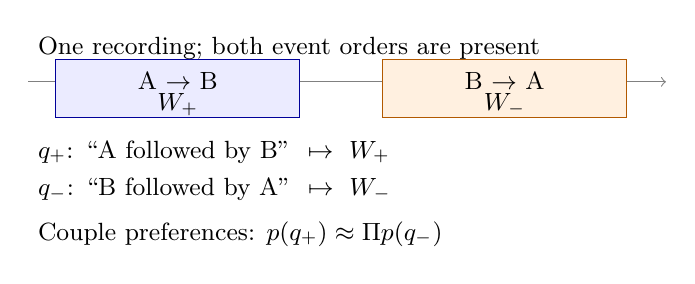
\begin{tikzpicture}[x=1cm,y=1cm,every node/.style={font=\small}]
\draw[->,gray] (0,1.65)--(8.1,1.65);
\node[anchor=west] at (0,2.08) {One recording; both event orders are present};
\draw[fill=blue!8,draw=blue!60!black] (0.35,1.2) rectangle (3.45,1.93);
\draw[fill=orange!12,draw=orange!70!black] (4.5,1.2) rectangle (7.6,1.93);
\node at (1.9,1.66) {A $\rightarrow$ B};
\node at (6.05,1.66) {B $\rightarrow$ A};
\node at (1.9,1.36) {$W_+$};
\node at (6.05,1.36) {$W_-$};
\node[anchor=west] at (0,0.76) {$q_+$: ``A followed by B'' $\ \mapsto\ W_+$};
\node[anchor=west] at (0,0.28) {$q_-$: ``B followed by A'' $\ \mapsto\ W_-$};
\node[anchor=west] at (0,-0.28) {Couple preferences: $p(q_+)\approx\Pi p(q_-)$};
\end{tikzpicture}
\caption{RelTwin schematic, not an observed test example. Both queries see the same waveform. Exchanging the relation changes the target window; the candidate preference vectors are compared after the corresponding permutation $\Pi$. Window layout is alternated across constructed recordings.}
\label{fig:pair}
\end{figure}
